%----------------------------------------------------------------------------------------
%	PACKAGES AND DOCUMENT CONFIGURATIONS
%----------------------------------------------------------------------------------------

\documentclass{article}

\usepackage[version=3]{mhchem} % Package for chemical equation typesetting
\usepackage{siunitx} % Provides the \SI{}{} and \si{} command for typesetting SI units
\usepackage{graphicx} % Required for the inclusion of images
\usepackage{natbib} % Required to change bibliography style to APA
\usepackage{amsmath} % Required for some math elements 
\usepackage{amssymb}
\graphicspath{ {./images/} }


\setlength\parindent{0pt} % Removes all indentation from paragraphs

\renewcommand{\labelenumi}{\alph{enumi}.} % Make numbering in the enumerate environment by letter rather than number (e.g. section 6)

%\usepackage{times} % Uncomment to use the Times New Roman font

%----------------------------------------------------------------------------------------
%	DOCUMENT INFORMATION
%----------------------------------------------------------------------------------------

\title{ASSIGNMENT 1: Fast Trajectory Planning} % Title, replace [N] with the current week number

\author{Erica Cai, Boning Ding, and Shreya Jahagirdar} % Author name

\date{\today} % Date for the report

\begin{document}

\maketitle % Insert the title, author and date



%----------------------------------------------------------------------------------------
%	SECTION 1
%----------------------------------------------------------------------------------------

\section*{0 Part 0 - Set Up Environments}

For our project, we performed each of Repeated Forward A* that breaks ties with larger g-values, Repeated Forward A* that breaks ties with smaller g-values, Repeated Backward A* that breaks ties with larger g-values, and Adaptive A* that breaks ties with larger g-values, on 50 gridworlds of size 101 x 101. The file 50Mazes.txt stores our gridworlds. \\

Each of our gridworlds has a ' ' to represent an unblocked cell and 'X' to represent a blocked cell. With 30\% probability, a cell is blocked, and with 70\% probability, a cell is unblocked. \\

For our experiments, we chose random start states and goal states, and verified that the start and goal states are unblocked. We also verified that the environment always has a path between the start state and goal state. Therefore, the A* search is always successful. \\

For each experiment of each algorithm, we also store the maze with the path that the agent follows to reach the goal state from the start state in [xxx].log files. These files also contain metadata about the algorithm's run on the maze, such as the start position, end position, total number of expanded cells, total number of searches, and the final agent path length. \\

We implemented our own binary heap to pop the nodes with the smallest f-values and to break ties for higher and lower g-values.
%----------------------------------------------------------------------------------------
%	SECTION 2
%----------------------------------------------------------------------------------------

\section{Part 1 - Understanding the Methods}

\subsection{Explain in your report why the first move of the agent for the example search problem from Figure 1  is to the east rather
than the north given that the agent does not know initially which cells are blocked.}

By definition, A* search will return the shortest path from A to T.\\

\begin{figure}[h!]
  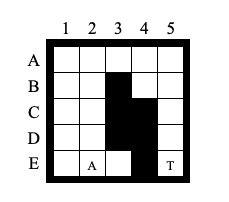
\includegraphics[width=0.5\textwidth]{p1_0.png}
  \caption{The actual grid }
\end{figure}

Initially, the agent does not know that any cells are blocked. Although the actual grid is shown in Figure 1, the agent perceives the grid to be as shown in Figure 2.  \\

\begin{figure}[h!]
  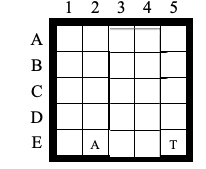
\includegraphics[]{p1_1.png}
  \caption{The agent's perspective of the grid }
\end{figure}

In this grid shown in Figure 2, the shortest path from  A to T is E2, E3, E4, E5. There is no path from A to T that is shorter. Since A* search returns the shortest path, A* search will return the path E2, E3, E4, E5.\\

Believing that Figure 2 is the grid, the agent will move along this path, first moving to the east, to E3. \\

We know that in the actual grid shown in Figure 1, the shortest path from A to T involves moving to the north first, to circumvent the obstacles, to get to T. However, the agent does not know that these obstacles exist. As a result, the agent will move to the east, believing that it is following a shorter path. \\

\subsection{Give a convincing argument that the agent in finite gridworlds indeed either reaches the target or discovers that this is impossible in finite time. }
We want to show 1. That the agent reaches the target in finite time, and 2. That the agent discovers that reaching the target is impossible in finite time. \\\\
1. Show that the agent reaches the target in finite time.
\begin{enumerate}
	\item If there is a path from the start state to the goal, then, if there is a path from the start state to state x, that means there is a path from state x to the goal (because the agent can go from state x, back to the start state, and then to the goal). Therefore, if there is a path from the start state to the goal, and a path from the start state to state x, then A* search can ALWAYS find a path from the state x to the goal. 
	\item After many A* searches, the agent will know the grid environment and will be able to find an unblocked path from the state x to the goal. The number of A* searches is finite because the agent will always begin the A* search at a block where it has not begun an A* search before. This is because the agent already knows how to navigate the environment of any cell that it has started an A* search at before.
	\item Therefore, the agent reaches the target after a finite number of A* searches. Each A* search is finite, so the agent reaches the target in finite time.
\end{enumerate}
2. Show that the agent discovers that reaching the target is impossible in finite time.
\begin{enumerate}
	\item If there is no path from the start state to the goal, then, if there is a path from the start state to state x, that means there is no path from state x to the goal (because the agent can go from state x, and back to the start state, realizing that it cannot reach the goal).
	\item After many A* searches, the agent will know the grid environment and realize that there is no path from the state x to the goal. The number of A* searches is finite because the agent will always begin the A* search at a block where it has not begun an A* search before. This is because the agent already knows how to navigate the environment of any cell that it has started an A* search at before.
	\item Therefore, the agent realizes that reaching the target is impossible after a finite number of A* searches. Each A* search is finite, so the agent discovers that reaching the target is impossible in finite time.
\end{enumerate}

\subsection{Prove that the number of moves of the agent until it reaches the target or discovers that this is impossible is bounded from above by the number of unblocked cells squared.}

We want to show 1. That the number of moves of the agent until it reaches the target is bounded above by the number of unblocked cells squared  2. That the number of moves that the agent makes before discovering that reaching the target is impossible is bounded above by the number of unblocked squared.\\

In either case, 
\begin{enumerate}
	\item The agent makes at most the number of unblocked cells moves after each A* search. This is because, in the worst case, the agent will traverse every unblocked cell in the grid. 
	\begin{enumerate}
		\item Show that the A* search will never return a path that is longer than the number of unblocked cells.  If the number of moves is more than the number of unblocked cells, that means the path that the A* search returns is more than the number of unblocked cells. This means, the path includes a state (i,j) twice, according to the pigeonhole principle. Therefore, the path has a cycle. As a result, the path is not the shortest path; a shorter path exists which has no cycles. Since A* search always returns the shortest path, it will never return a path that is longer than the number of unblocked cells.
	\end{enumerate}
	\item The number of A* searches that the agent makes is at most the number of unblocked cells.
	\begin{enumerate}
		\item Show that the agent will always begin an A* search at a cell where it has not begun an A* search before.  The agent already knows how to navigate the environment of any cell that it has started an A* search at before. Therefore, it will not get blocked in a cell that it has started an A* search at before. As a result, it will not start an A* search at a cell that it has started at before. 
		\item Show that the number of A* searches that the agent makes cannot be more than the number of unblocked cells. The agent can only start a search at an unblocked cell. We know from part (a) that an agent will always begin an A* search where it has not begun an A* search before. Therefore, the agent must start the search at an unblocked cell that it has not started at before, and in the worst case, the agent will start the search the number of unblocked cells times.
	\end{enumerate} 
\end {enumerate}
Since the agent makes at most the number of unblocked cells moves after each A* search, and the number of A* searches that the agent makes is at most the number of blocked cells, the number of moves that the agent makes is the number of unblocked cells * the number of unblocked cells, which is the number of unblocked cells squared.\\

We have just showed that the maximum number of moves that the agent can make is bounded by the number of unblocked cells squared. In part 2.2, we also showed that the agent reaches the target or discovers that this is impossible in finite time. Since the maximum number of moves is bounded by the number of unblocked cells squared, then the number of moves of the agent until it reaches the target or discovers that this is impossible is bounded from above by the number of unblocked cells squared.

%----------------------------------------------------------------------------------------
%	SECTION 3
%----------------------------------------------------------------------------------------

\section{Part 2 - The Effects of Ties}

\subsection{Implement and compare both versions of Repeated Forward A* with respect to their runtime or, equivalently, number of expanded cells.}
 The next page contains a table, Table 1, comparing both versions of Repeated Forward A*, with respect to their number of expanded cells.\\
\begin{table}
\centering
\resizebox{\textwidth}{!}{\begin{tabular}{||p{1.5cm}|p{1.5cm}|p{1.5cm}|p{3.5cm}|p{3.5cm}||}
%\begin{tabular}{||p{1.5cm}|p{1.5cm}|p{1.5cm}|p{3.5cm}|p{3.5cm}||}
 \hline
 Trial & Start State & End State & Number of Total Expanded Nodes for Repeated Forward A* Breaking Ties with Larger G Values & Number of Total Expanded Nodes for Repeated Forward A* Breaking Ties with Smaller G Values \\ [0.5ex] 
 \hline\hline
 Maze 1 & (0,0) & (97,96) & 15398 & 415754 \\ 
 \hline
Maze 2 & (53,13) & (40,38) & 509 & 3332\\
 \hline
 Maze 3 & (91,11) & (51,64) & 2728 & 30555\\
 \hline
 Maze 4 & (78,91) & (89,11) & 4865 & 19385\\  
 \hline
 Maze 5 & (96,83) & (68,94) & 320 & 1807\\
 \hline
 Maze 6 & (2,76) & (96,20) & 8737 & 156826\\
 \hline
 Maze 7 & (3,83) & (79,6) & 4780 & 89176 \\ 
 \hline
 Maze 8 & (44,35) & (44,85) & 277 & 500\\
 \hline
 Maze 9 & (84,95) & (12,21) & 12643 & 302673\\
 \hline
 Maze 10 & (97,94) & (14,18) & 13911 & 341722\\
 \hline
 Maze 11 & (11,70) & (6,87) & 296 & 707\\
 \hline
 Maze 12 & (10,10) & (85,24) & 3012 & 12236\\ 
 \hline
 Maze 13 & (8,92) & (40,75) & 631 & 3470 \\
 \hline
  Maze 14 & (42,92) & (34,57) & 302 & 1323 \\
 \hline
 Maze 15 & (65,20) & (97,68) & 1093 & 8989\\
 \hline
 Maze 16 & (49,64) & (49,86) & 122 & 218\\
 \hline
 Maze 17 & (28,50) & (85,11) & 2812 & 29626\\
 \hline
 Maze 18 & (36,28) & (91,86) & 2608 & 45597\\
 \hline
 Maze 19 & (94,35) & (58,62) & 828 & 4362\\ 
 \hline
 Maze 20 & (21,9) & (11,16) & 96 & 298 \\
 \hline
 Maze 21 & (16,68) & (84,3) & 11583 & 279185\\
 \hline
 Maze 22 & (78,37) & (37,30) & 1630 & 6142\\
 \hline
 Maze 23 & (56,14) & (61,13) & 6 & 11\\
 \hline
 Maze 24 & (96,35) & (10,49) & 4324 & 19573\\ 
 \hline
 Maze 25 & (59,35) & (85,78) & 3020 & 35466\\
 \hline
  Maze 26 & (44,73) & (33,57) & 251 & 832\\
 \hline
 Maze 27 & (55,80) & (79,18) & 2081& 20471 \\
 \hline
 Maze 28 & (84,22) & (12,73) & 4953 & 92956 \\
 \hline
 Maze 29 & (26,36) & (42,46) & 103 & 535 \\
 \hline
 Maze 30 & (63,92) & (45,46) & 2064 & 22572 \\
 \hline
 Maze 31 & (81,21) & (57,22) & 189 & 477\\ 
 \hline
 Maze 32 & (46,1) & (18,73) & 2606 & 30785\\
 \hline
 Maze 33 & (21,80) & (27,71) & 75 & 217 \\
 \hline
 Maze 34 & (18,85) & (79,16) & 7315 & 158493\\
 \hline
 Maze 35 & (16,99) & (38,4) & 10680 & 134222 \\
 \hline
 Maze 36 & (12,82) & (84,25) & 4982 & 76851\\ 
 \hline
 Maze 37 & (89,17) & (79,55) & 710 & 2717\\
 \hline
  Maze 38 & (5,15) & (70,72) & 5741 & 87633 \\
 \hline
 Maze 39 & (59,100) & (68,83) & 922 & 2659\\
 \hline
 Maze 40 & (76,85) & (7,12) & 10035 & 224726\\
 \hline
 Maze 41 & (67,96) & (36,52) & 1778 & 22698 \\
 \hline
 Maze 42 & (52,50) & (83,11) & 1085 & 10728 \\
 \hline
 Maze 43 & (70,39) & (23,57) & 3442 & 20433\\ 
 \hline
 Maze 44 & (29,44) & (23,52) & 119 & 326 \\
 \hline
 Maze 45 & (1,50) & (82,98) & 5953 & 55863 \\
 \hline
 Maze 46 & (15,3) & (87,29) & 5535 & 44318 \\
 \hline
 Maze 47 &  (34,45) & (86,65)& 2174 & 15773\\ 
 \hline
 Maze 48 & (51,100) & (90,50)  & 2089 & 29515\\
 \hline
 Maze 49 & (34,15) & (2,28) & 2137 & 6481\\
 \hline
 Maze 50 & (7,82) & (69,27) & 9805 & 186701\\
\hline
Total & n/a & n/a & 183355 & 3057915
\\[.3ex]
 \hline
\end{tabular}}
\caption{Comparison of the Number of Total Expanded Nodes using Repeated Forward A* that Breaks Ties with Larger G-Values and Repeated Forward A* that Breaks Ties with Smaller G-Values on 50 Trials } 
\end{table} 

From Table 1, we observe that the version of Repeated Forward A* which breaks ties with larger g-values expands much fewer nodes than the version of Repeated Forward A* that breaks ties with smaller g-values, in every trial. Therefore, the version of Repeated Forward A* that breaks ties with larger g-values will run much more quickly than the version of Repeated Forward A* that breaks ties with smaller g-values.\\\\\\\\\\\\\\

\subsection{Explain your observations in detail, that is, explain what you observed and give a reason for the observation.}

For our explanation, let two nodes, n and m, have the same f value.\\\\
According to the f value equation, we know

\[f_n = g_n + h_n \]
\[f_m = g_m + h_m \]

Assume that
\[f_n = f_m \]
\[g_n > g_m \]

Given these four equations, we know that
\[h_n<h_m\]

By definition, the h-value is an estimate of the distance between a node and the goal. Since node n has a smaller h-value than node m, then node n is closer to the goal than node m. Therefore, the agent is choosing to expand the node that is closer to the goal.\\\\
The node that is closer to the goal has a higher chance of being on the shortest path because there is a smaller distance to travel before reaching the goal.



%----------------------------------------------------------------------------------------
%	SECTION 4
%----------------------------------------------------------------------------------------

\section{Part 3 - Forward vs. Backward}


\subsection{Implement and compare Repeated Forward A* and Repeated Backward A* with respect to their runtime or, equivalently, number of expanded cells. }
The next page contains a table, Table 2, comparing Repeated Forward A* and Repeated Backward A*, with respect to their number of expanded cells.\\


From Table 2, we observe that the version of Repeated Forward A* which breaks ties with larger g-values expands much fewer nodes than the version of Repeated Backward A* that breaks ties with larger g-values, in every trial. Therefore, the version of Repeated Forward A* that breaks ties with larger g-values will run much more quickly than the version of Repeated Backward A* that breaks ties with larger g-values.
\begin{table}
\centering
\resizebox{\textwidth}{!}{\begin{tabular}{||p{1.5cm}|p{1.5cm}|p{1.5cm}|p{3.5cm}|p{3.5cm}||}
%\begin{tabular}{||p{1.5cm}|p{1.5cm}|p{1.5cm}|p{3.5cm}|p{3.5cm}||}
 \hline
 Trial & Start State & End State & Number of Total Expanded Nodes for Repeated Forward A* Breaking Ties with Larger G Values & Number of Total Expanded Nodes for Repeated Backward A* Breaking Ties with Larger G Values \\ [0.5ex] 
 \hline\hline
 Maze 1 & (0,0) & (97,96) & 15398 & 389367 \\ 
 \hline
Maze 2 & (53,13) & (40,38) & 509 & 514\\
 \hline
 Maze 3 & (91,11) & (51,64) & 2728 & 31181\\
 \hline
 Maze 4 & (78,91) & (89,11) & 4865 & 14653\\  
 \hline
 Maze 5 & (96,83) & (68,94) & 320 & 876\\
 \hline
 Maze 6 & (2,76) & (96,20) & 8737 & 53524\\
 \hline
 Maze 7 & (3,83) & (79,6) & 4780 & 28188 \\ 
 \hline
 Maze 8 & (44,35) & (44,85) & 277 & 539\\
 \hline
 Maze 9 & (84,95) & (12,21) & 12643 & 123905\\
 \hline
 Maze 10 & (97,94) & (14,18) & 13911 & 169511\\
 \hline
 Maze 11 & (11,70) & (6,87) & 296 & 375\\
 \hline
 Maze 12 & (10,10) & (85,24) & 3012 & 2455\\ 
 \hline
 Maze 13 & (8,92) & (40,75) & 631 & 6587 \\
 \hline
  Maze 14 & (42,92) & (34,57) & 302 & 2657 \\
 \hline
 Maze 15 & (65,20) & (97,68) & 1093 & 16969\\
 \hline
 Maze 16 & (49,64) & (49,86) & 122 & 190\\
 \hline
 Maze 17 & (28,50) & (85,11) & 2812 & 25245\\
 \hline
 Maze 18 & (36,28) & (91,86) & 2608 & 37641\\
 \hline
 Maze 19 & (94,35) & (58,62) & 828 & 9818\\ 
 \hline
 Maze 20 & (21,9) & (11,16) & 96 & 2151\\
 \hline
 Maze 21 & (16,68) & (84,3) & 11583 & 158854\\
 \hline
 Maze 22 & (78,37) & (37,30) & 1630 & 10207\\
 \hline
 Maze 23 & (56,14) & (61,13) & 6 & 6\\
 \hline
 Maze 24 & (96,35) & (10,49) & 4324 & 18750\\ 
 \hline
 Maze 25 & (59,35) & (85,78) & 3020 & 22624\\
 \hline
  Maze 26 & (44,73) & (33,57) & 251 & 381\\
 \hline
 Maze 27 & (55,80) & (79,18) & 2081& 15739 \\
 \hline
 Maze 28 & (84,22) & (12,73) & 4953 & 49164 \\
 \hline
 Maze 29 & (26,36) & (42,46) & 103 & 556 \\
 \hline
 Maze 30 & (63,92) & (45,46) & 2064 & 9815 \\
 \hline
 Maze 31 & (81,21) & (57,22) & 189 & 310\\ 
 \hline
 Maze 32 & (46,1) & (18,73) & 2606 & 21385\\
 \hline
 Maze 33 & (21,80) & (27,71) & 75 & 178 \\
 \hline
 Maze 34 & (18,85) & (79,16) & 7315 & 47587\\
 \hline
 Maze 35 & (16,99) & (38,4) & 10680 & 125877 \\
 \hline
 Maze 36 & (12,82) & (84,25) & 4982 & 20463\\ 
 \hline
 Maze 37 & (89,17) & (79,55) & 710 & 2267\\
 \hline
  Maze 38 & (5,15) & (70,72) & 5741 & 23791 \\
 \hline
 Maze 39 & (59,100) & (68,83) & 922 & 3792\\
 \hline
 Maze 40 & (76,85) & (7,12) & 10035 & 51845\\
 \hline
 Maze 41 & (67,96) & (36,52) & 1778 & 5787 \\
 \hline
 Maze 42 & (52,50) & (83,11) & 1085 & 4897 \\
 \hline
 Maze 43 & (70,39) & (23,57) & 3442 & 19597\\ 
 \hline
 Maze 44 & (29,44) & (23,52) & 119 & 2149 \\
 \hline
 Maze 45 & (1,50) & (82,98) & 5953 & 19210 \\
 \hline
 Maze 46 & (15,3) & (87,29) & 5535 & 35242 \\
 \hline
 Maze 47 &  (34,45) & (86,65)& 2174 & 14754\\ 
 \hline
 Maze 48 & (51,100) & (90,50)  & 2089 & 3862\\
 \hline
 Maze 49 & (34,15) & (2,28) & 2137 & 4170\\
 \hline
 Maze 50 & (7,82) & (69,27) & 9805 & 81607\\
\hline
Total & n/a & n/a & 183355 & 1689212
\\[.3ex]
 \hline
\end{tabular}}
\caption{Comparison of the Number of Total Expanded Nodes using Repeated Forward A* that Breaks Ties with Larger G-Values and Repeated Backward A* that Breaks Ties with Larger G-Values on 50 Trials} 
\end{table} 

\subsection{Explain your observations in detail, that is, explain what you observed and give a reason for the observation.}
For our explanation, let the agent perceive the grid to be as in Figure 3. In the grid, let A be the agent's current location and T be the target.\\

\begin{figure}[h!]
  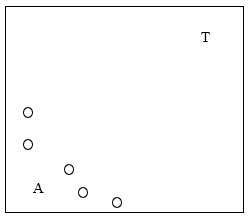
\includegraphics[width=0.5\textwidth]{p3_0.png}
  \caption{The agent's perception of the grid }
\end{figure}

The grid in Figure 3 is an accurate representation of an agent's perception of the grid because the agent knows the environment of cells that are close to it. However, the agent does not know the environment of cells that are far from it, such as for the cells that are close to T.\\

\begin{figure}[h!]
  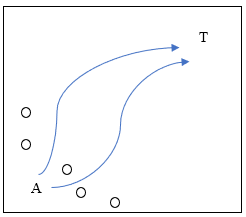
\includegraphics[width=0.5\textwidth]{p3_1.png}
  \caption{Possibilities for shortest paths from the agent to the target in Repeated Forward A*}
\end{figure}

The A* search in Repeated Forward A* will search for a path from the start node to the goal node. At the beginning of the search, the agent A will see that there are not many possibilities for paths to the target T, so the agent's search tree will be very small. An example of the possibilities of paths that the agent may explore is in Figure 4.\\

\begin{figure}[h!]
  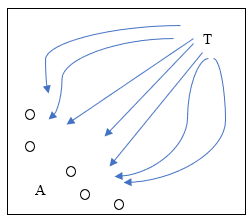
\includegraphics[width=0.5\textwidth]{p3_2.png}
  \caption{Possibilities for shortest paths from the target to the agent in Repeated Backward A*}
\end{figure}


On the other hand, the A* search in Repeated Backward A* will search for a path from the goal node to the start node. At the beginning of the search, the target T sees many possibilities for paths to the agent A, since the agent does not perceive many blocked cells around the target T. As a result, the agent's search tree will be much larger than in Repeated Forward A*. An example of the possibilities of paths that the agent may explore is in Figure 5. \\

Since the agent explores many more paths in Repeated Backward A* than in Repeated Forward A*, the agent spends more time to examine those paths. As a result, Repeated Backward A* is usually slower than Repeated Forward A*.

%----------------------------------------------------------------------------------------
%	SECTION 5
%----------------------------------------------------------------------------------------

\section{Part 4 - Heuristics in the Adaptive A*}

\subsection{Prove that “the Manhattan distances are consistent in gridworlds in which the agent can move only in the four main compass directions.”}
For a node n, a neighbor $n_0$, and action a, the definition of consistency is \[ \forall (n,a,n_0): h(n) \leq  c(n,a,n_0)+h(n_0)\]

Show that this is true, given that the h-value is the Manhattan distance, and the agent can move only in the four main compass directions.\\

Let the coordinates of n to be $(x_n,y_n)$.\\
Let the coordinates of $n_0$ to be $(x_{n_0},y_{n_0})$.\\
Let the coordinates of the goal, g, to be $(x_g,y_g)$.\\

By the definition of the heuristic function,
\[ h(n)=|x_g-x_n|+|y_g-y_n|\]
\[ h(n_0)=|x_g-x_{n_0}|+|y_g-y_{n_0}|\]

Also, since the agent can move only in the four main compass directions
\[ c(n,a,n_0)=|x_{n_0}-x_n|+|y_{n_0}-y_n|\]

Next, the following are true because of $|x+y|\leq|x|+|y|$
\[ |x_g-x_{n_0}+x_{n_0}-x_n|=|x_g-x_n|\leq|x_g-x_{n_0}|+|x_{n_0}-x_n| \]
\[ |y_g-y_{n_0}+y_{n_0}-y_n|=|y_g-y_n|\leq|y_g-y_{n_0}|+|y_{n_0}-y_n| \]

Therefore, by adding the above inequalities together,
\[ h(n)=|x_g-x_n|+|y_g-y_n|\leq|x_g-x_{n_0}|+|y_g-y_{n_0}|+|x_{n_0}-x_n|+|y_{n_0}-y_n| \]

Which, by definition, means
\[h(n)\leq c(n,a,n_0)+h(n_0) \] 

Since n may be any node and $n_0$ may be any neighbor of n, the Manhattan distances are consistent in gridwords in which the agent can move only in the four main compass directions.

\[ \forall (n,a,n_0): h(n) \leq  c(n,a,n_0)+h(n_0)\]

\subsection{Prove that Adaptive A* leaves initially consistent h-values consistent even if action costs can increase.}

For a node n, a neighbor $n_0$, and action a, the definition of consistency is \[ \forall (n,a,n_0): h(n) \leq  c(n,a,n_0)+h(n_0)\]

To show that this is true for Adaptive A*, first, prove that the g-value of the goal is greater than the g-value of any node in the closed list. We will use the claim from the first proof to prove that the h-values are consistent.

\begin{itemize}
	\item Proof 1. Prove that $g(goal) \geq g(n) $ . Let goal be the goal state and let n be any node that is in the closed list before reaching that goal state.\\
	
	We know that n is any node in the closed list. Let n' be the next node after n has been explored that is on the optimal path from the start state to the goal state, as shown in Figure 6.

	\begin{figure}[h!]
  		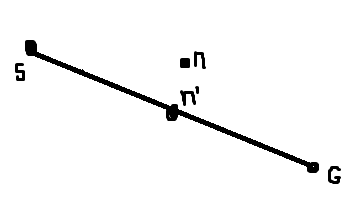
\includegraphics[width=0.5\textwidth]{p4_0.png}
 		 \caption{Illustration of n and n' . Let the black line be the optimal path from the start to the goal state.}
	\end{figure}

	The f-value of n is less than or equal to the f-value of n' since we assume n to be in the closed list before n' was added to it. Therefore,
	\[ g(n)+h(n) \leq g(n')+h(n') \]
	 Also, we know that the f-value of the node n' is less than or equal to the f-value of the goal, by definition of the A* algorithm. Further, the f-value of the goal is the same as the g-value of the goal, since the h-value of the goal is 0. Therefore, 
	\[g(n') +h(n') \leq f(goal)=g(goal) \]
	Putting the inequalities together, 
	\[g(n)+h(n) \leq g(goal) \]
	\[g(n) \leq g(goal) \]

	\item Proof 2. Use the claim from proof 1 to prove that the h-values from the Adaptive A* algorithm are consistent, that $ \forall (n,a,n_0): h(n) \leq  c(n,a,n_0)+h(n_0)$
	
	Let n be a node, $n_0$ be a neighbor of node n, and a be an action.
	By the definition of the heuristic function for adaptive A*, 
	\[h(n)=g(goal)-g(n) \]
	\[h(n_0)=g(goal)-g(n_0) \]
	Because of proof 1, which proves that difference between g-value of the goal and the g-value of any node in the closed list is always positive
	\[h(n)=|g(goal)-g(n)| \]
	\[h(n_0)=|g(goal)-g(n_0)| \]
	Since n is a neighbor of $n_0$ ,
	\[c(n,a,n_0)=|g(n_0)-g(n)|=1 \]
	The following is true because of $|x+y|\leq|x|+|y|$
	\[|g(goal)-g(n_0)+g(n_0)-g(n)| \leq |g(goal)-g(n_0)|+|g(n_0)-g(n)| \]
	Therefore, 
	\[ h(n)= |g(goal)-g(n)| = |g(goal)-g(n_0)+g(n_0)-g(n)|  \]
	\[ \leq |g(goal)-g(n_0)|+|g(n_0)-g(n)|=h(n_0)+c(n,a,n_0) \]
	Since n may be any node and $n_0$ may be any neighbor of n, heuristics are consistent in the Adaptive A* algorithm.
	\[ \forall (n,a,n_0): h(n) \leq  c(n,a,n_0)+h(n_0)\]

\end{itemize}




%----------------------------------------------------------------------------------------
%	SECTION 5
%----------------------------------------------------------------------------------------

\section{Part 5 - Heuristics in the Adaptive A*}

\subsection{ Implement and compare Repeated Forward A* and Adaptive A* with respect to their runtime.}

The next page contains a table, Table 3, comparing Repeated Forward A* and  Adaptive A*, with respect to their number of expanded cells.\\
\begin{table}
\centering
\resizebox{\textwidth}{!}{\begin{tabular}{||p{1.5cm}|p{1.5cm}|p{1.5cm}|p{3.5cm}|p{3.5cm}||}
%\begin{tabular}{||p{1.5cm}|p{1.5cm}|p{1.5cm}|p{3.5cm}|p{3.5cm}||}
 \hline
 Trial & Start State & End State & Number of Total Expanded Nodes for Repeated Forward A* Breaking Ties with Larger G Values & Number of Total Expanded Nodes for Adaptive A* Breaking Ties with Larger G Values \\ [0.5ex] 
 \hline\hline
 Maze 1 & (0,0) & (97,96) & 15398 & 14556 \\ 
 \hline
Maze 2 & (53,13) & (40,38) & 509 & 423\\
 \hline
 Maze 3 & (91,11) & (51,64) & 2728 & 2308\\
 \hline
 Maze 4 & (78,91) & (89,11) & 4865 & 4884\\  
 \hline
 Maze 5 & (96,83) & (68,94) & 320 & 302\\
 \hline
 Maze 6 & (2,76) & (96,20) & 8737 & 8542\\
 \hline
 Maze 7 & (3,83) & (79,6) & 4780 & 4779 \\ 
 \hline
 Maze 8 & (44,35) & (44,85) & 277 & 276\\
 \hline
 Maze 9 & (84,95) & (12,21) & 12643 & 12474\\
 \hline
 Maze 10 & (97,94) & (14,18) & 13911 & 13896\\
 \hline
 Maze 11 & (11,70) & (6,87) & 296 & 274\\
 \hline
 Maze 12 & (10,10) & (85,24) & 3012 & 2764\\ 
 \hline
 Maze 13 & (8,92) & (40,75) & 631 & 607 \\
 \hline
  Maze 14 & (42,92) & (34,57) & 302 & 301 \\
 \hline
 Maze 15 & (65,20) & (97,68) & 1093 & 1040\\
 \hline
 Maze 16 & (49,64) & (49,86) & 122 & 122\\
 \hline
 Maze 17 & (28,50) & (85,11) & 2812 & 2749\\
 \hline
 Maze 18 & (36,28) & (91,86) & 2608 & 2591\\
 \hline
 Maze 19 & (94,35) & (58,62) & 828 & 609\\ 
 \hline
 Maze 20 & (21,9) & (11,16) & 96 & 96 \\
 \hline
 Maze 21 & (16,68) & (84,3) & 11583 & 11540\\
 \hline
 Maze 22 & (78,37) & (37,30) & 1630 & 1605\\
 \hline
 Maze 23 & (56,14) & (61,13) & 6 & 6\\
 \hline
 Maze 24 & (96,35) & (10,49) & 4324 & 4296\\ 
 \hline
 Maze 25 & (59,35) & (85,78) & 3020 & 2983\\
 \hline
  Maze 26 & (44,73) & (33,57) & 251 & 239\\
 \hline
 Maze 27 & (55,80) & (79,18) & 2081& 2053 \\
 \hline
 Maze 28 & (84,22) & (12,73) & 4953 & 4051 \\
 \hline
 Maze 29 & (26,36) & (42,46) & 103 & 103 \\
 \hline
 Maze 30 & (63,92) & (45,46) & 2064 & 2051 \\
 \hline
 Maze 31 & (81,21) & (57,22) & 189 & 160\\ 
 \hline
 Maze 32 & (46,1) & (18,73) & 2606 & 2580\\
 \hline
 Maze 33 & (21,80) & (27,71) & 75 & 75 \\
 \hline
 Maze 34 & (18,85) & (79,16) & 7315 & 7220\\
 \hline
 Maze 35 & (16,99) & (38,4) & 10680 & 10487 \\
 \hline
 Maze 36 & (12,82) & (84,25) & 4982 & 4905\\ 
 \hline
 Maze 37 & (89,17) & (79,55) & 710 & 694\\
 \hline
  Maze 38 & (5,15) & (70,72) & 5741 & 4781 \\
 \hline
 Maze 39 & (59,100) & (68,83) & 922 & 686\\
 \hline
 Maze 40 & (76,85) & (7,12) & 10035 & 9939\\
 \hline
 Maze 41 & (67,96) & (36,52) & 1778 & 1777 \\
 \hline
 Maze 42 & (52,50) & (83,11) & 1085 & 1072 \\
 \hline
 Maze 43 & (70,39) & (23,57) & 3442 & 3335\\ 
 \hline
 Maze 44 & (29,44) & (23,52) & 119 & 114 \\
 \hline
 Maze 45 & (1,50) & (82,98) & 5953 & 5924 \\
 \hline
 Maze 46 & (15,3) & (87,29) & 5535 & 5318 \\
 \hline
 Maze 47 &  (34,45) & (86,65)& 2174 & 2141\\ 
 \hline
 Maze 48 & (51,100) & (90,50)  & 2089 & 2086\\
 \hline
 Maze 49 & (34,15) & (2,28) & 2137 & 2073\\
 \hline
 Maze 50 & (7,82) & (69,27) & 9805 & 9681\\
\hline
Total & n/a & n/a & 183355 & 177568
\\[.3ex]
 \hline
\end{tabular}}
\caption{Comparison of the Number of Total Expanded Nodes using Repeated Forward A* that Breaks Ties with Larger G-Values and Adaptive A* that Breaks Ties with Larger G-Values on 50 Trials} 
\end{table} 

From Table 3, we observe that the version of Repeated Forward A* which breaks ties with larger g-values usually expands more nodes than the version of Repeated Backward A* that breaks ties with larger g-values, in the trials. Therefore, the version of Repeated Forward A* that breaks ties with larger g-values will usually run more slowly than the version of Repeated Backward A* that breaks ties with larger g-values.

\subsection{Explain your observations in detail, that is, explain what you observed and give a reason for the observation.}
Our explanation involves the definition of the heuristic function for both algorithms.\\

By definition, the heuristic function is an estimate of the distance from the current state to the goal state. The h-value in the adaptive A* algorithm is always equal to or greater than the h-value in the Repeated Forward A* algorithm, which is always the Manhattan distance.  \\

However, the heuristic function in Adaptive A* is admissible. Therefore, the h-value of a node is always less than the actual shortest distance from the node to the goal state.\\

Since the h-value in Adaptive A* is greater than or equal to that of Repeated Forward A*, it is more accurate than that of Repeated Forward A*. \\

As a result, the f-values of some nodes, whose path to the goal is long due to many blocked cells, will be higher, and those nodes will be correctly less likely to be expanded from the open list.\\


%----------------------------------------------------------------------------------------
%	SECTION 5
%----------------------------------------------------------------------------------------

\section{Part 6 - Memory Issues}

\subsection{Suggest additional ways to reduce the memory consumption of your implementations further.}

Some important information we first need to gather would be how much memory Python allocates for different data structures. We can use the code below to give us an idea about what data structures to use for our more optimized implementation.

\begin{figure}[h!]
  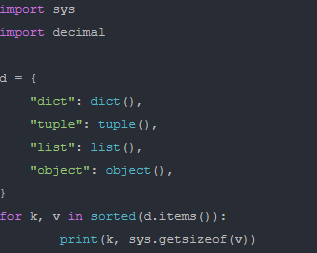
\includegraphics[width=0.5\textwidth]{p6_0.png}
  \caption{Code that determines the size of data structures in Python }
\end{figure}

Using this small script, we will get the following byte sizes for each data structure\\
dict: 248\\
list: 72\\
object: 16\\
tuple: 56\\

The first step in optimizing our memory would be to use tuples whenever possible, limit our usage of lists, and completely avoid dictionaries. Instead of using arrays for coordinates, we can use tuples instead. Therefore, for the agent to keep track of the grid, we can have a 3d array with tuples as coordinates to keep track of the positions as well as any flags that lets the agent know what the cell is (3 elements. 1. isBlocked, 2. lastSeen, 3. heuristicValue). Furthermore, we will have an array for the open list, closed list, and path. Although the path and open list can be ignored as this list is relatively small and are reinitialized after every iteration of our search.\\

Although the open list is reinitialized during each iteration of A* search, we can still consider saving some memory during runtime by skipping the node objects that are blocked. This will allow us to make our memory 30\% more efficient assuming an ideal grid world has 30\% blocked nodes and 70\% open nodes.\\

Another way that we can save memory is by saving bits. Since we keep track of whether a cell is blocked by storing an integer 0, 1, or 2, we can use two bits to store whether that cell is blocked, rather than use an entire integer that takes up 4 bytes in Python. We can use 2 bits instead of the 4 bytes because we can store 0 as bits 00, 1 as bits 01, and 2 as bits 10. 


\subsection{Calculate the amount of memory that they need to operate on gridworlds of size 1001 x 1001 and the largest gridworld that they can operate on within a memory limit of 4 MBytes.}

Knowing this information, we can make the calculations required for the question to part 6.\\\\
For the calculations, we add up the memory that we use to store information about the board and the maximum amount of memory that we use to store nodes in the open or closed list.\\\\
From the script that was we can start with the entire grid world which contains\\
\[ 1001 * 1001 = 1002001 \] 
cells. \\\\
1. To store information about the board, we have a 2 dimensional array with cells that correspond to each state of the maze. In each cell, we will have a list with 3 integer elements: one to indicate whether the state is a blocked state, the second to indicate during which search that state was most recently explored, and the last to indicate the heuristic value of the state, if there is one. So the board uses
\[72 + (1001 * 72) + 1002001 * (72 + 3 * 16) = 120.31\]
MB. The 72 is for the total array, the 1001* 72 is for the subarrays at each row of the total array, and the 1002001 * (72 + 3 * 16)  is for the subarrays in each cell of the 2d array. \\

2. Now we calculate the memory for the closed list and the open list. Say that our worst case results in the closed list and open list together storing 90\% of the node objects. Since it is a single array, we will get the memory usage of 
\[0.9 * 1002001 * (16 * 6)) + 72 +72 = 86.57 \]
MB, by applying the formula: 90\% of the total gridworld * total size of grid world * size of the node object + size of closed list structure + size of open list structure. The node object contains the g value, h-value, f-value, and x and y coordinate ( instead of a tuple; two objects require less space than a tuple. So we can do an x and y value for the node))\\

Adding both of these together, we will get 
\[120.31 + 86.57 = 206.88\]
MB for a 1001x1001 grid world.\\

For 4MB limited space, we can solve the equation\\
\[ ((0.9 * \lfloor x^2 \rfloor) * (16 * 6)) + 72+72) + (\lfloor x^2 \rfloor * (72 + 3 * 16) + (1001 * 72) + 72) = 4000000\]
 bytes.
\[x = 137\]
Therefore, the best we can do with 4MB would be a 137x137 grid.





\end{document}